% Options for packages loaded elsewhere
\PassOptionsToPackage{unicode}{hyperref}
\PassOptionsToPackage{hyphens}{url}
%
\documentclass[
  letterpaper,
]{scrbook}

\usepackage{amsmath,amssymb}
\usepackage{iftex}
\ifPDFTeX
  \usepackage[T1]{fontenc}
  \usepackage[utf8]{inputenc}
  \usepackage{textcomp} % provide euro and other symbols
\else % if luatex or xetex
  \usepackage{unicode-math}
  \defaultfontfeatures{Scale=MatchLowercase}
  \defaultfontfeatures[\rmfamily]{Ligatures=TeX,Scale=1}
\fi
\usepackage{lmodern}
\ifPDFTeX\else  
    % xetex/luatex font selection
\fi
% Use upquote if available, for straight quotes in verbatim environments
\IfFileExists{upquote.sty}{\usepackage{upquote}}{}
\IfFileExists{microtype.sty}{% use microtype if available
  \usepackage[]{microtype}
  \UseMicrotypeSet[protrusion]{basicmath} % disable protrusion for tt fonts
}{}
\makeatletter
\@ifundefined{KOMAClassName}{% if non-KOMA class
  \IfFileExists{parskip.sty}{%
    \usepackage{parskip}
  }{% else
    \setlength{\parindent}{0pt}
    \setlength{\parskip}{6pt plus 2pt minus 1pt}}
}{% if KOMA class
  \KOMAoptions{parskip=half}}
\makeatother
\usepackage{xcolor}
\setlength{\emergencystretch}{3em} % prevent overfull lines
\setcounter{secnumdepth}{5}
% Make \paragraph and \subparagraph free-standing
\ifx\paragraph\undefined\else
  \let\oldparagraph\paragraph
  \renewcommand{\paragraph}[1]{\oldparagraph{#1}\mbox{}}
\fi
\ifx\subparagraph\undefined\else
  \let\oldsubparagraph\subparagraph
  \renewcommand{\subparagraph}[1]{\oldsubparagraph{#1}\mbox{}}
\fi


\providecommand{\tightlist}{%
  \setlength{\itemsep}{0pt}\setlength{\parskip}{0pt}}\usepackage{longtable,booktabs,array}
\usepackage{calc} % for calculating minipage widths
% Correct order of tables after \paragraph or \subparagraph
\usepackage{etoolbox}
\makeatletter
\patchcmd\longtable{\par}{\if@noskipsec\mbox{}\fi\par}{}{}
\makeatother
% Allow footnotes in longtable head/foot
\IfFileExists{footnotehyper.sty}{\usepackage{footnotehyper}}{\usepackage{footnote}}
\makesavenoteenv{longtable}
\usepackage{graphicx}
\makeatletter
\def\maxwidth{\ifdim\Gin@nat@width>\linewidth\linewidth\else\Gin@nat@width\fi}
\def\maxheight{\ifdim\Gin@nat@height>\textheight\textheight\else\Gin@nat@height\fi}
\makeatother
% Scale images if necessary, so that they will not overflow the page
% margins by default, and it is still possible to overwrite the defaults
% using explicit options in \includegraphics[width, height, ...]{}
\setkeys{Gin}{width=\maxwidth,height=\maxheight,keepaspectratio}
% Set default figure placement to htbp
\makeatletter
\def\fps@figure{htbp}
\makeatother
\newlength{\cslhangindent}
\setlength{\cslhangindent}{1.5em}
\newlength{\csllabelwidth}
\setlength{\csllabelwidth}{3em}
\newlength{\cslentryspacingunit} % times entry-spacing
\setlength{\cslentryspacingunit}{\parskip}
\newenvironment{CSLReferences}[2] % #1 hanging-ident, #2 entry spacing
 {% don't indent paragraphs
  \setlength{\parindent}{0pt}
  % turn on hanging indent if param 1 is 1
  \ifodd #1
  \let\oldpar\par
  \def\par{\hangindent=\cslhangindent\oldpar}
  \fi
  % set entry spacing
  \setlength{\parskip}{#2\cslentryspacingunit}
 }%
 {}
\usepackage{calc}
\newcommand{\CSLBlock}[1]{#1\hfill\break}
\newcommand{\CSLLeftMargin}[1]{\parbox[t]{\csllabelwidth}{#1}}
\newcommand{\CSLRightInline}[1]{\parbox[t]{\linewidth - \csllabelwidth}{#1}\break}
\newcommand{\CSLIndent}[1]{\hspace{\cslhangindent}#1}

\makeatletter
\makeatother
\makeatletter
\@ifpackageloaded{bookmark}{}{\usepackage{bookmark}}
\makeatother
\makeatletter
\@ifpackageloaded{caption}{}{\usepackage{caption}}
\AtBeginDocument{%
\ifdefined\contentsname
  \renewcommand*\contentsname{Table of contents}
\else
  \newcommand\contentsname{Table of contents}
\fi
\ifdefined\listfigurename
  \renewcommand*\listfigurename{List of Figures}
\else
  \newcommand\listfigurename{List of Figures}
\fi
\ifdefined\listtablename
  \renewcommand*\listtablename{List of Tables}
\else
  \newcommand\listtablename{List of Tables}
\fi
\ifdefined\figurename
  \renewcommand*\figurename{Figure}
\else
  \newcommand\figurename{Figure}
\fi
\ifdefined\tablename
  \renewcommand*\tablename{Table}
\else
  \newcommand\tablename{Table}
\fi
}
\@ifpackageloaded{float}{}{\usepackage{float}}
\floatstyle{ruled}
\@ifundefined{c@chapter}{\newfloat{codelisting}{h}{lop}}{\newfloat{codelisting}{h}{lop}[chapter]}
\floatname{codelisting}{Listing}
\newcommand*\listoflistings{\listof{codelisting}{List of Listings}}
\makeatother
\makeatletter
\@ifpackageloaded{caption}{}{\usepackage{caption}}
\@ifpackageloaded{subcaption}{}{\usepackage{subcaption}}
\makeatother
\makeatletter
\makeatother
\ifLuaTeX
  \usepackage{selnolig}  % disable illegal ligatures
\fi
\IfFileExists{bookmark.sty}{\usepackage{bookmark}}{\usepackage{hyperref}}
\IfFileExists{xurl.sty}{\usepackage{xurl}}{} % add URL line breaks if available
\urlstyle{same} % disable monospaced font for URLs
\hypersetup{
  pdftitle={Fundamentals of Biodiversity Data Science},
  pdfauthor={Timothée Poisot},
  hidelinks,
  pdfcreator={LaTeX via pandoc}}

\title{Fundamentals of Biodiversity Data Science}
\author{Timothée Poisot}
\date{2023-08-05}

\begin{document}
\frontmatter
\maketitle
\renewcommand*\contentsname{Table of contents}
{
\setcounter{tocdepth}{1}
\tableofcontents
}
\mainmatter
\bookmarksetup{startatroot}

\hypertarget{preface}{%
\chapter*{Preface}\label{preface}}
\addcontentsline{toc}{chapter}{Preface}

\markboth{Preface}{Preface}

This is a Quarto book.

To learn more about Quarto books visit
\url{https://quarto.org/docs/books}.

\bookmarksetup{startatroot}

\hypertarget{introduction}{%
\chapter{Introduction}\label{introduction}}

Data science is now an established methodology to study biodiversity,
and this is a problem. Well, this is an opportunity when it comes to
advancing our knowledge of biodiversity (Tuia et al. 2022), but this is
a problem for us, biodiversity scientists, as we suddenly need to
develop competences in an entirely new field. And as luck would have it,
there are easier fields to master than data science.

But what do we mean by \emph{data science}? Most science, after all,
relies on data in some capacity. What falls under the umbrella of data
science is, in short, embracing in equal measure quantitative skills
(mathematics, machine learning, statistics), programming, and domain
expertise, in order to solve well-defined problems. A core tenet of data
science is that, when using it, we seek to ``deliver actionable
insights'', which is MBA-speak for ``figuring out what to do next''. One
of the ways in which this occurs is by letting the data speak, after
they have been, of course, properly cleaned and transformed and
engineered beyond recognition.

Before we embark into a journey of discovery on the applications of data
science to biodiversity, allow me to let you in on a little secret. Data
\emph{science} is a little bit of a misnomer. Science is (or so we like
to say) neutral, systematic, and rigorous. Science is baking. Data
science? It's cooking. There might be a recipe, but it's a
recommendation at best,and after all you know better than to follow a
list of instructions, don't you? Data science is craft. It's art. Data
vibes.

\bookmarksetup{startatroot}

\hypertarget{creating-groups-the-k-means-algorithm}{%
\chapter{\texorpdfstring{Creating groups: the \emph{k}-means
algorithm}{Creating groups: the k-means algorithm}}\label{creating-groups-the-k-means-algorithm}}

As we mentioned in the introduction, a core idea of data science is that
things that look the same (in that, when described with data, they
resemble one another) are likely to be the same. Although this sounds
like a simplifying assumption, this can provide the basis for a very
powerful technique in which we \emph{create} groups in data that have no
labels. This task is called unsupervised clustering: we seek to add a
\emph{label} to each observation, in order to form groups, and the data
we work from do \emph{not} have a label that we can use to train a
model.

\hypertarget{a-digression-which-birds-are-red}{%
\section{A digression: which birds are
red?}\label{a-digression-which-birds-are-red}}

Before diving in, it is a good idea to ponder a simple case. We can
divide everything in just two categories: things with red feathers, and
things without red feathers. An example of a thing with red feathers is
the Northern Cardinal (\emph{Cardinalis cardinalis}), and an example of
things without red feathers are the iMac G3, Haydn's string quartets,
and of course the Northern Cardinal (\emph{Cardinalis cardinalis}).

See, biodiversity data science is complicated, because it tends to rely
on the assumption that we can categorize the natural world, and the
natural world (mostly in response to natural selection) comes up with
ways to be, well, diverse. In the Northern Cardinal, this is shown in
males having red feathers, and females having mostly brown feathers.
Before moving forward, we need to consider ways to solve this issue, as
this issue will come up \emph{all the time.}

The first mistake we have made is that the scope of objects we want to
classify, which we will describe as the ``domain'' of our
classification, is much too broad: there are few legitimate applications
where we will have a dataset with Northern Cardinals, iMac G3s, and
Haydn's string quartets. Picking a reasonable universe of classes would
have solved our problem a little. For example, among the things that do
not have red feathers are the Mourning Dove, the Kentucky Warbler, and
the House Sparrow.

The second mistake that we have made is improperly defining our classes;
bird species exhibit sexual dimorphism (not in an interesting way, like
wrasses, but you let's still give them some credit for trying). Assuming
that there is such a thing as a Northern Cardinal is not necessarily a
reasonable assumption! And yet, the assumption that a single label is a
valid representation of non-monomorphic populations is a surprisingly
common one, with actual consequences for the performance of image
classification algorithms (Luccioni and Rolnick 2023). This assumption
reveals a lot about our biases: male specimens are over-represented in
museum collections, for example (Cooper et al. 2019). In a lot of
species, we would need to split the taxonomic unit into multiple groups
in order to adequately describe them.

The third mistake we have made is using predictors that are too vague.
The ``presence of red feathers'' is not a predictor that can easily
discriminate between the Northen Cardinal (yes for males, sometimes for
females), the House Finch (a little for males, no for females), and the
Red-Winged Black Bird (a little for males, no for females). In fact, it
cannot really capture the difference between red feathers for the male
House Finch (head and breast) and the male Red Winged Black Bird (wings,
as the name suggests).

The final mistake we have made is in assuming that ``red'' is relevant
as a predictor. In a wonderful paper, Cooney et al. (2022) have
converted the color of birds into a bird-relevant colorimetric space,
revealing a clear latitudinal trend in the ways bird colors, as
perceived by other birds, are distributed. This analysis, incidentally,
splits all species into males and females. The use of a color space that
accounts for the way colors are perceived is a fantastic example of why
data science puts domain knowledge front and center.

Deciding which variables are going to be accounted for, how the labels
will be defined, and what is considered to be within or outside the
scope of the classification problem is \emph{difficult}. It requires
domain knowledge (you must know a few things about birds in order to
establish criteria to classify birds), and knowledge of how the
classification methods operate (in order to have just the right amount
of overlap between features in order to provide meaningful estimates of
distance).

\hypertarget{the-problem-classifying-pixels-from-an-image}{%
\section{The problem: classifying pixels from an
image}\label{the-problem-classifying-pixels-from-an-image}}

Throughout this chapter, we will work on a single image -- we may
initially balk at the idea that an image is data, but it is!
Specifically, an image is a series of instances (the pixels), each
described by their position in a multidimensional colorimetric space.
Greyscale images have one dimension, and images in color (like the one
we use here) will have three: their red, green, and blue channels. Not
only are images data, this specific dataset is going to be far larger
than many of the datasets we will work on in practice: the number of
pixels we work with is given by the product of the width and height of
the image!

\begin{figure}

{\centering 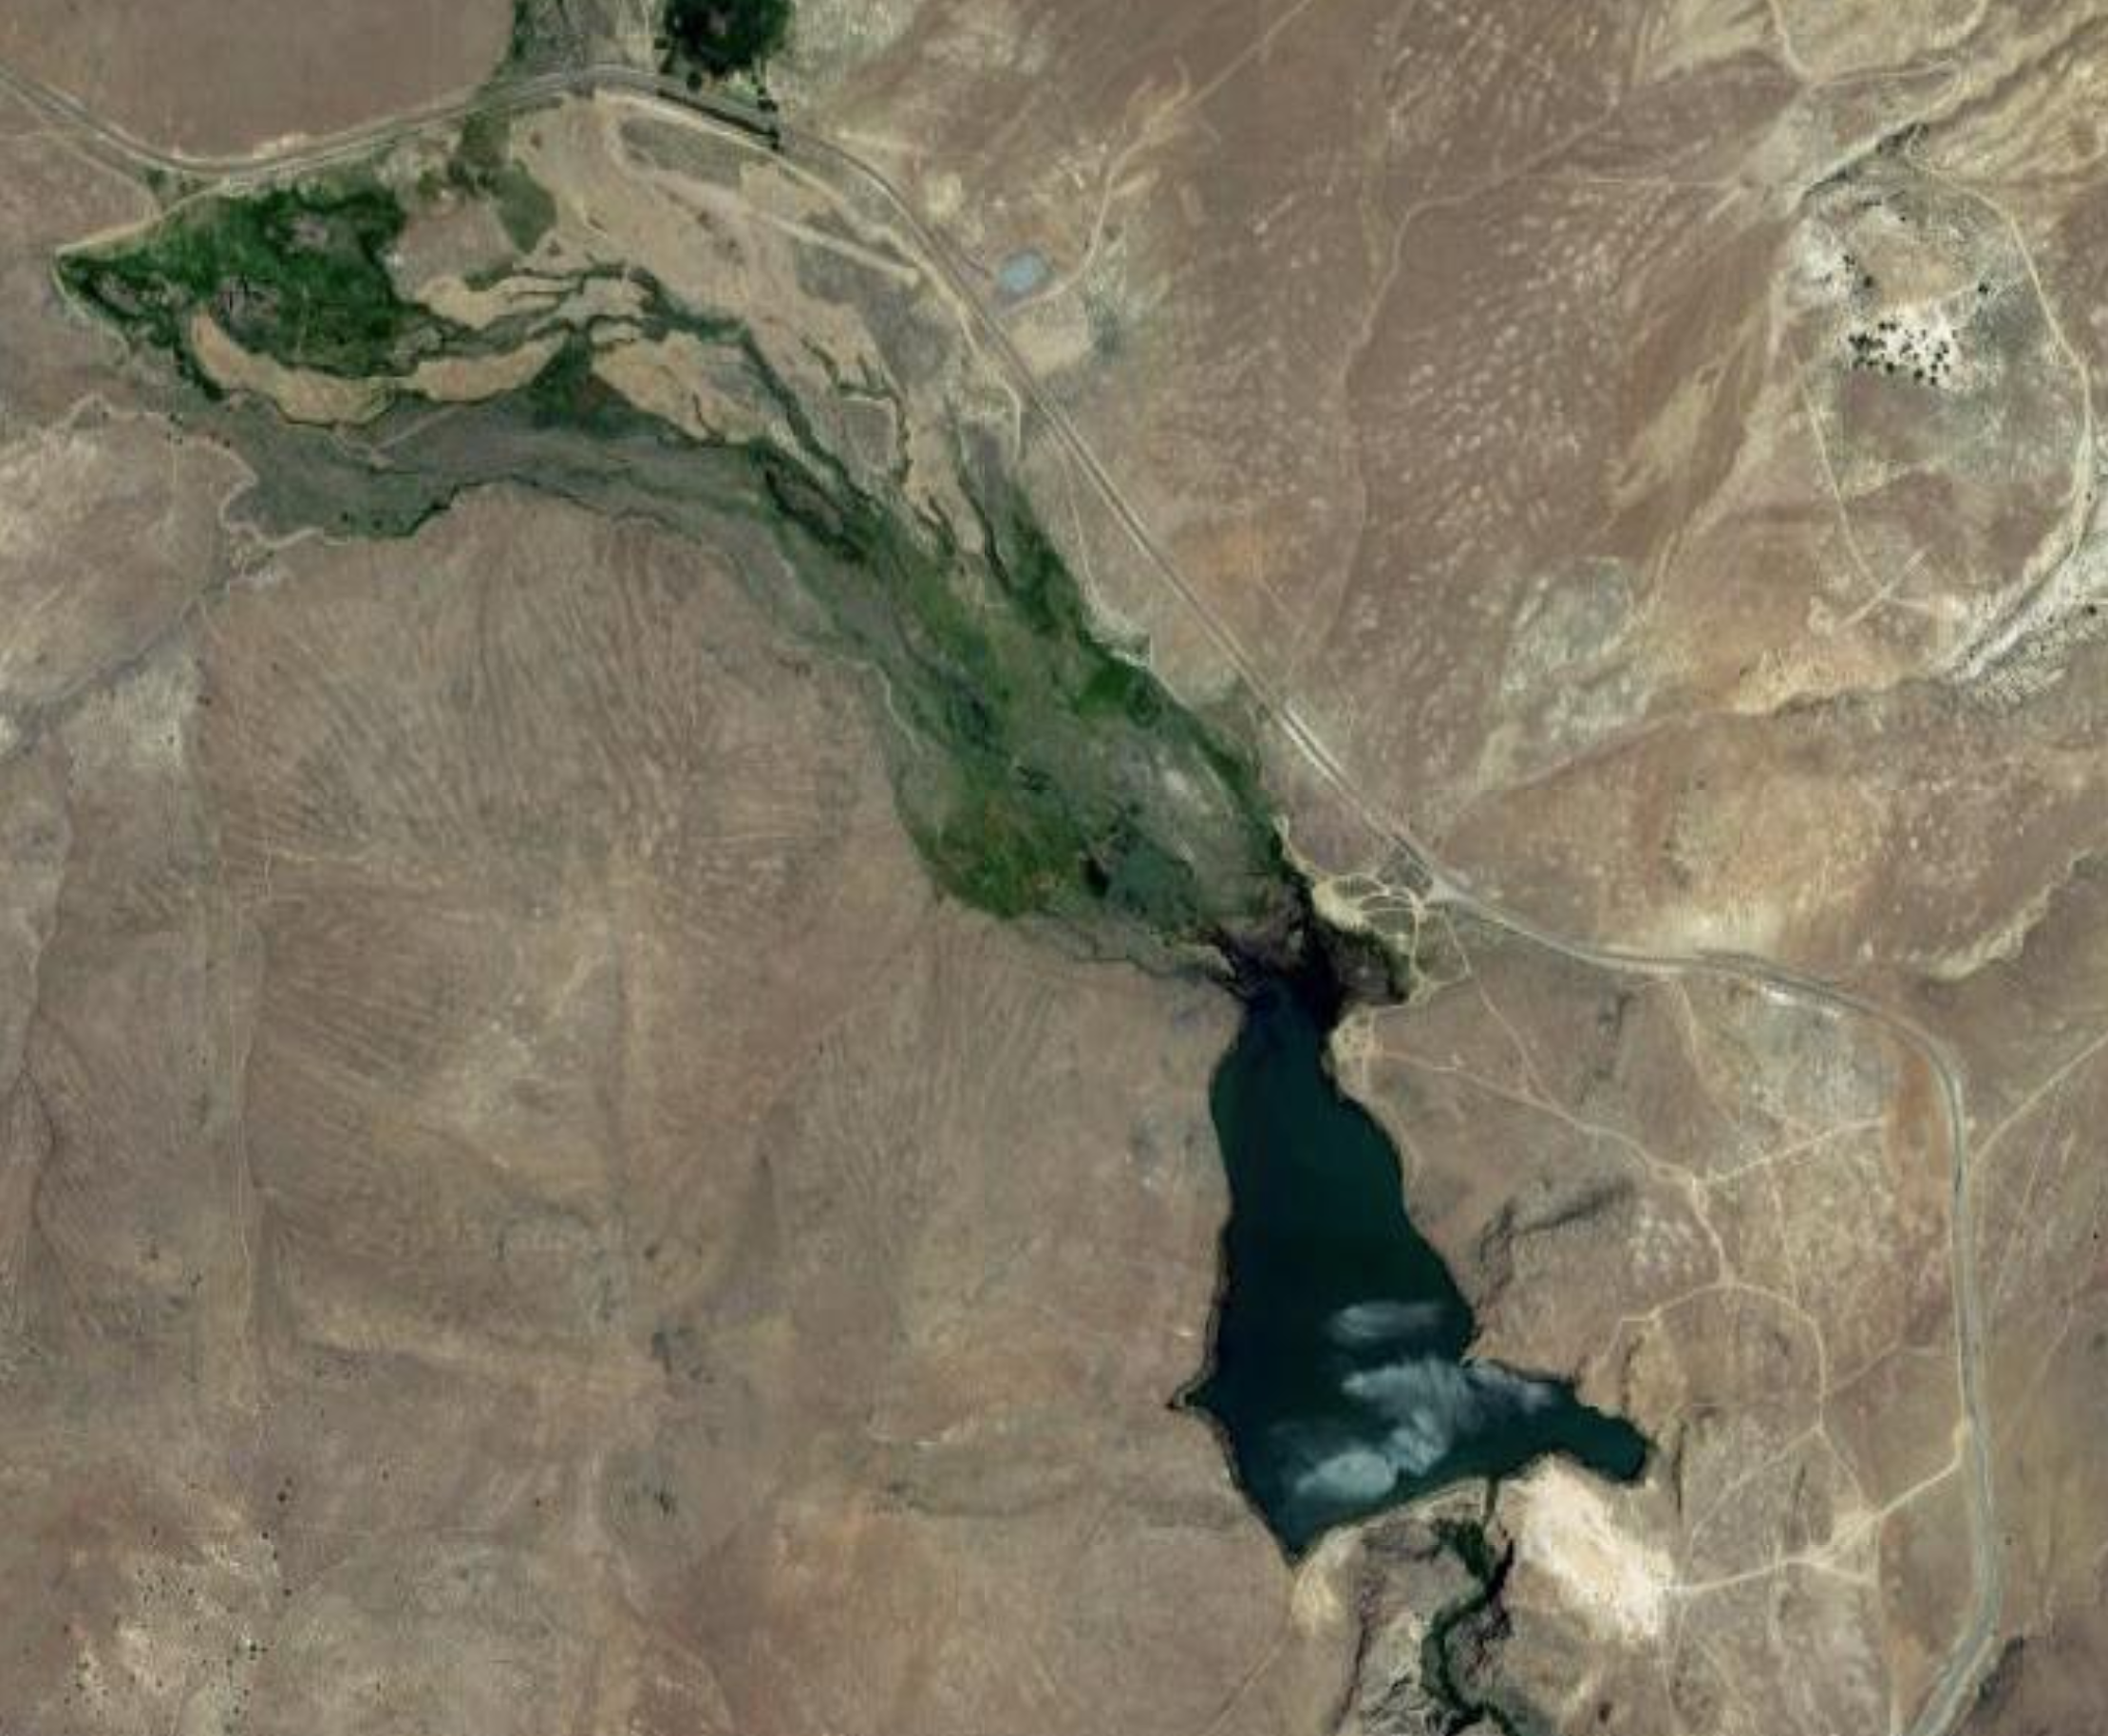
\includegraphics{data/kmeans/landscape.png}

}

\caption{This satellite image is made of pixels, each of which can be
represented as vector of red, green, and blue values. By finding groups
of pixels with similar positions in the colorimetric space, we hope to
highlight regions of the landscape that are similar.}

\end{figure}

We can decompose this image to have a look at the relationship between
the red and green channels, for example:

\begin{figure}

{\centering 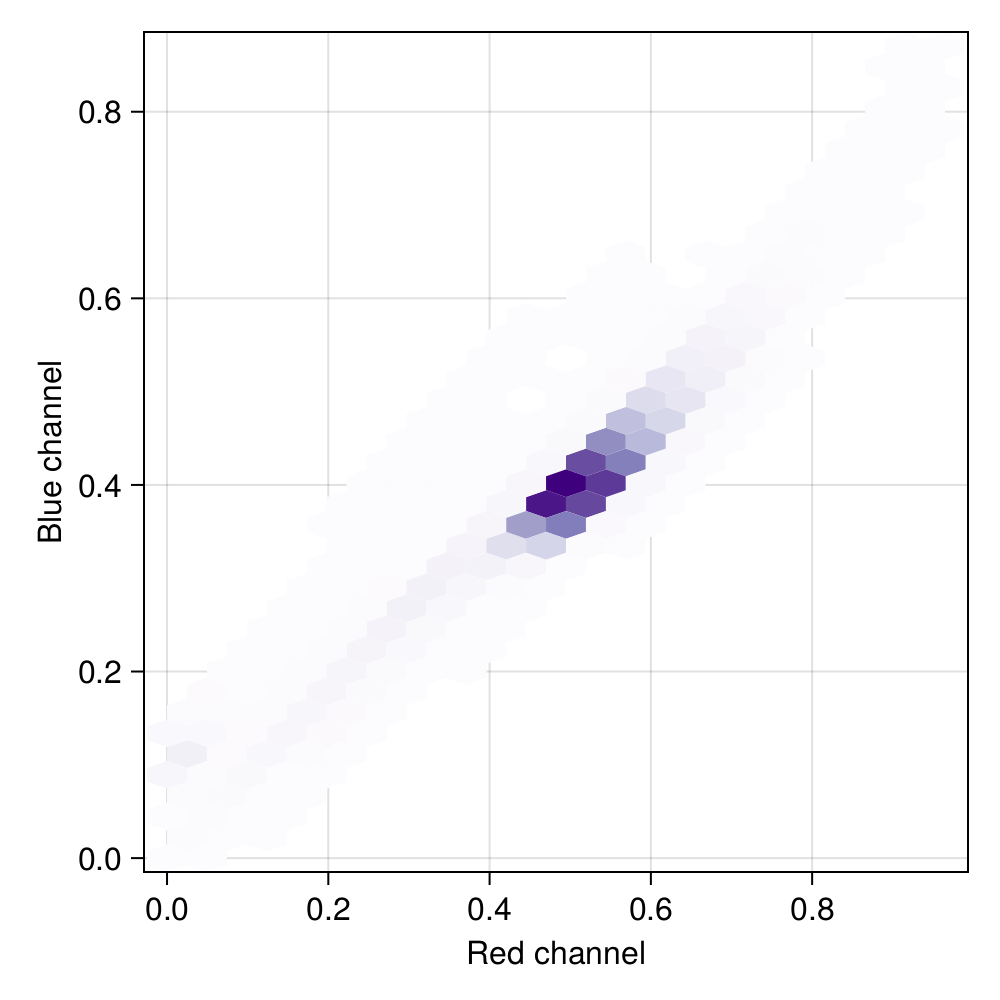
\includegraphics{chapters/kmeans_files/figure-latex/fig-hexbin-output-1.png}

}

\caption{\label{fig-hexbin}The pixels in the image exist in a
three-dimensional space representing their red, green, and blue values.
Hopefully, there is enough signal in this information to extract groups
of pixels that represent the same type of land cover.}

\end{figure}

\hypertarget{the-theory-behind-k-means-clustering}{%
\section{\texorpdfstring{The theory behind \emph{k}-means
clustering}{The theory behind k-means clustering}}\label{the-theory-behind-k-means-clustering}}

In order to understand the theory underlying \emph{k}-means, we will
work backwards from its output. As a method for unsupervised clustering,
\emph{k}-means will return a vector of \emph{class memberships}, which
is to say, a list that maps each observation (pixel, in our case) to a
class (tentatively, a cohesive landscape unit). What this means is that
\emph{k}-means is a transformation, taking as its input a vector with
three dimensions (red, green, blue), and returning a scalar (an integer,
even!), giving the class to which this pixel belongs. These are the
input and output of our blackbox, and now we can start figuring out its
internals.

\hypertarget{overview-of-the-algorithms}{%
\subsection{Overview of the
algorithms}\label{overview-of-the-algorithms}}

\hypertarget{identification-of-the-optimal-number-of-clusters}{%
\section{Identification of the optimal number of
clusters}\label{identification-of-the-optimal-number-of-clusters}}

\hypertarget{application-optimal-clustering-of-the-satellite-image-data}{%
\section{Application: optimal clustering of the satellite image
data}\label{application-optimal-clustering-of-the-satellite-image-data}}

\begin{figure}

{\centering 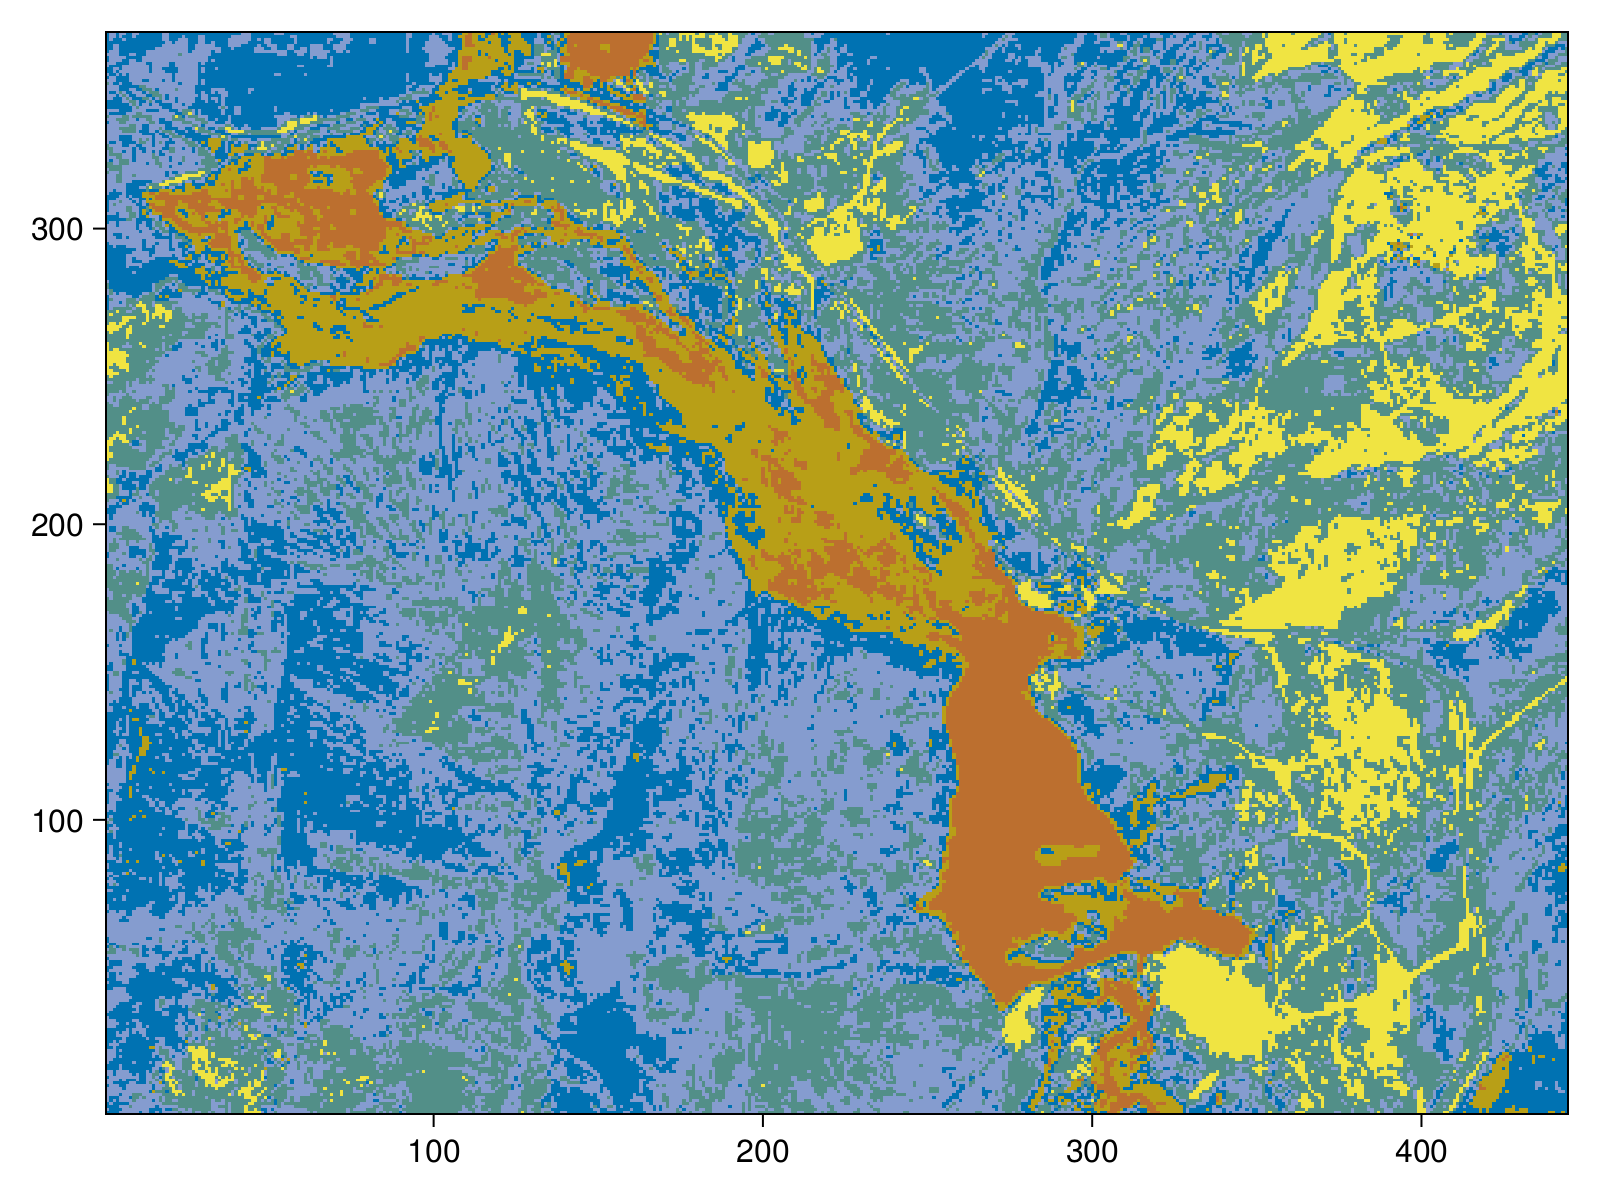
\includegraphics{chapters/kmeans_files/figure-latex/fig-classified-landscape-output-1.png}

}

\caption{\label{fig-classified-landscape}After iterating the
\emph{k}-means algorithm, \ldots{}}

\end{figure}

\hypertarget{alternatives-and-improvements}{%
\section{Alternatives and
improvements}\label{alternatives-and-improvements}}

EM

k-median

k-medoids

\bookmarksetup{startatroot}

\hypertarget{minimizing-error-the-gradient-descent-algorithm}{%
\chapter{Minimizing error: the gradient descent
algorithm}\label{minimizing-error-the-gradient-descent-algorithm}}

https://www.kaggle.com/datasets/abrambeyer/openintro-possum

\bookmarksetup{startatroot}

\hypertarget{summary}{%
\chapter{Summary}\label{summary}}

In summary, this book has no content whatsoever.

\bookmarksetup{startatroot}

\hypertarget{references}{%
\chapter*{References}\label{references}}
\addcontentsline{toc}{chapter}{References}

\markboth{References}{References}

\hypertarget{refs}{}
\begin{CSLReferences}{1}{0}
\leavevmode\vadjust pre{\hypertarget{ref-cooney2022}{}}%
Cooney, Christopher R., Yichen He, Zoë K. Varley, Lara O. Nouri,
Christopher J. A. Moody, Michael D. Jardine, András Liker, Tamás
Székely, and Gavin H. Thomas. 2022. {``Latitudinal Gradients in Avian
Colourfulness.''} \emph{Nature Ecology \& Evolution} 6 (5): 622--29.
\url{https://doi.org/10.1038/s41559-022-01714-1}.

\leavevmode\vadjust pre{\hypertarget{ref-cooper2019}{}}%
Cooper, Natalie, Alexander L. Bond, Joshua L. Davis, Roberto Portela
Miguez, Louise Tomsett, and Kristofer M. Helgen. 2019. {``Sex Biases in
Bird and Mammal Natural History Collections.''} \emph{Proceedings of the
Royal Society B: Biological Sciences} 286 (1913): 20192025.
\url{https://doi.org/10.1098/rspb.2019.2025}.

\leavevmode\vadjust pre{\hypertarget{ref-luccioni2023}{}}%
Luccioni, Alexandra Sasha, and David Rolnick. 2023. {``Bugs in the Data:
How ImageNet Misrepresents Biodiversity.''} \emph{Proceedings of the
AAAI Conference on Artificial Intelligence} 37 (12): 14382--90.
\url{https://doi.org/10.1609/aaai.v37i12.26682}.

\leavevmode\vadjust pre{\hypertarget{ref-tuia2022}{}}%
Tuia, Devis, Benjamin Kellenberger, Sara Beery, Blair R. Costelloe,
Silvia Zuffi, Benjamin Risse, Alexander Mathis, et al. 2022.
{``Perspectives in Machine Learning for Wildlife Conservation.''}
\emph{Nature Communications} 13 (1): 792.
\url{https://doi.org/10.1038/s41467-022-27980-y}.

\end{CSLReferences}


\backmatter

\end{document}
